\textbf{Date:} June 3th 2014\\\textbf{Duration:} 9-12\\\textbf{Group
members:} Henrik, Jakob, Jesper

\subsection{Goals for today}

\begin{itemize}
\itemsep1pt\parskip0pt\parsep0pt
\item
  Finalize new robot prototype build.
\item
  Have it follow the track using the line follower + tacho turner.
\item
  Get a first run going!
\end{itemize}

\subsection{Results}

Today went with building the new prototype, which we have ready for
action. The mechanism is working fine, although we still need a way to
hold onto the the solar panels.\\We have the robot following lines, and
rotating almost 90 degrees.

\begin{figure}[hbt]
  \centering
  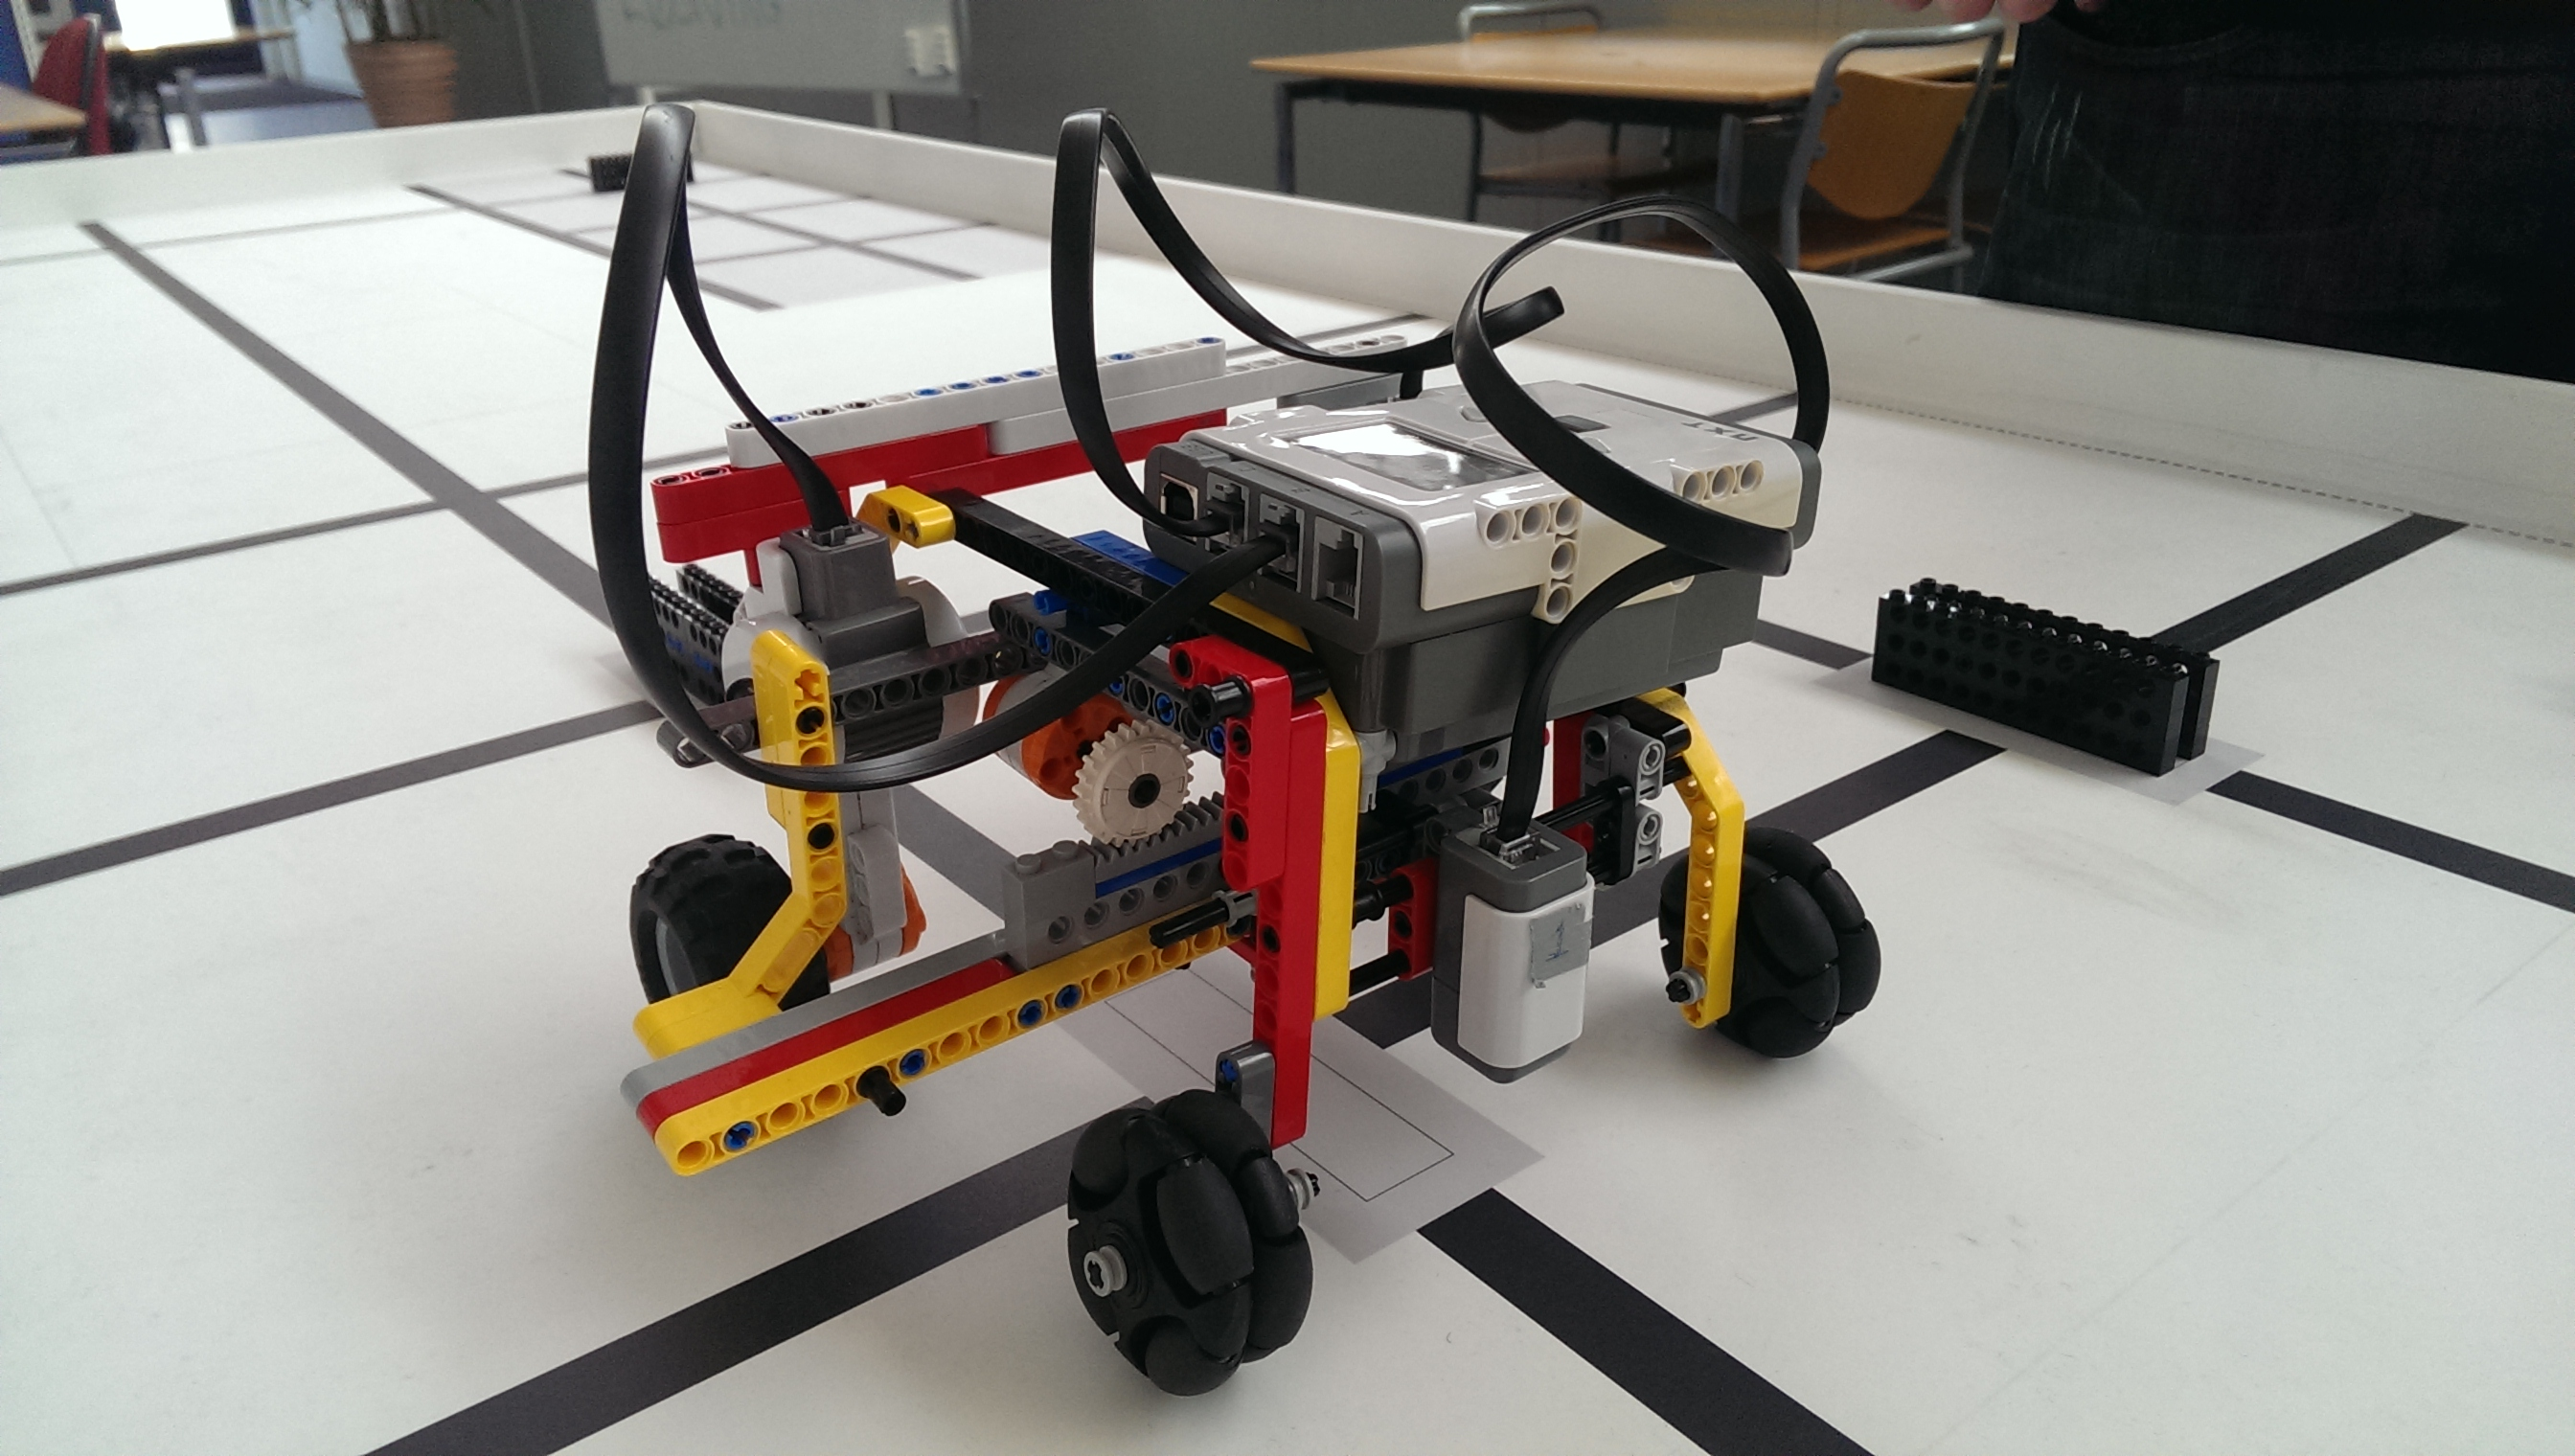
\includegraphics[scale=0.1]{../experiments/images/simplePrototype.jpg}
\caption{Picture of our prototype.}
\end{figure}

\subsection{Conclusion}
Today's meeting came to an early end as one member had to go, and we
decided to postpone the full track run for tomorrow.
